\section[氦原子]{氦原子} \label{sec:10.03} % 
% \makebox[5em][s]{} % 短题目拉间距

如果忽略原子核的运动,氦原子可以当作二电子体系,如图\ref{fig.10-1},体系的总能量包括电子的动能,原子核(电荷$2e$)对电子的库仑作用势能,以及两电子间库仑作用势能,
\eqlong
\begin{empheq}{equation}\label{eqx3.1}
	H=-\frac{\hbar^{2}}{2m_{e}}(\nabla_{1}^{2}+\nabla_{2}^{2})-\frac{2\e^{2}}{r_{1}}-\frac{2\e^{2}}{r_{2}}+\frac{\e^{2}}{r_{12}}
\end{empheq}\eqlong
\begin{wrapfigure}[10]{r}{9em}
	\centering
	\small
	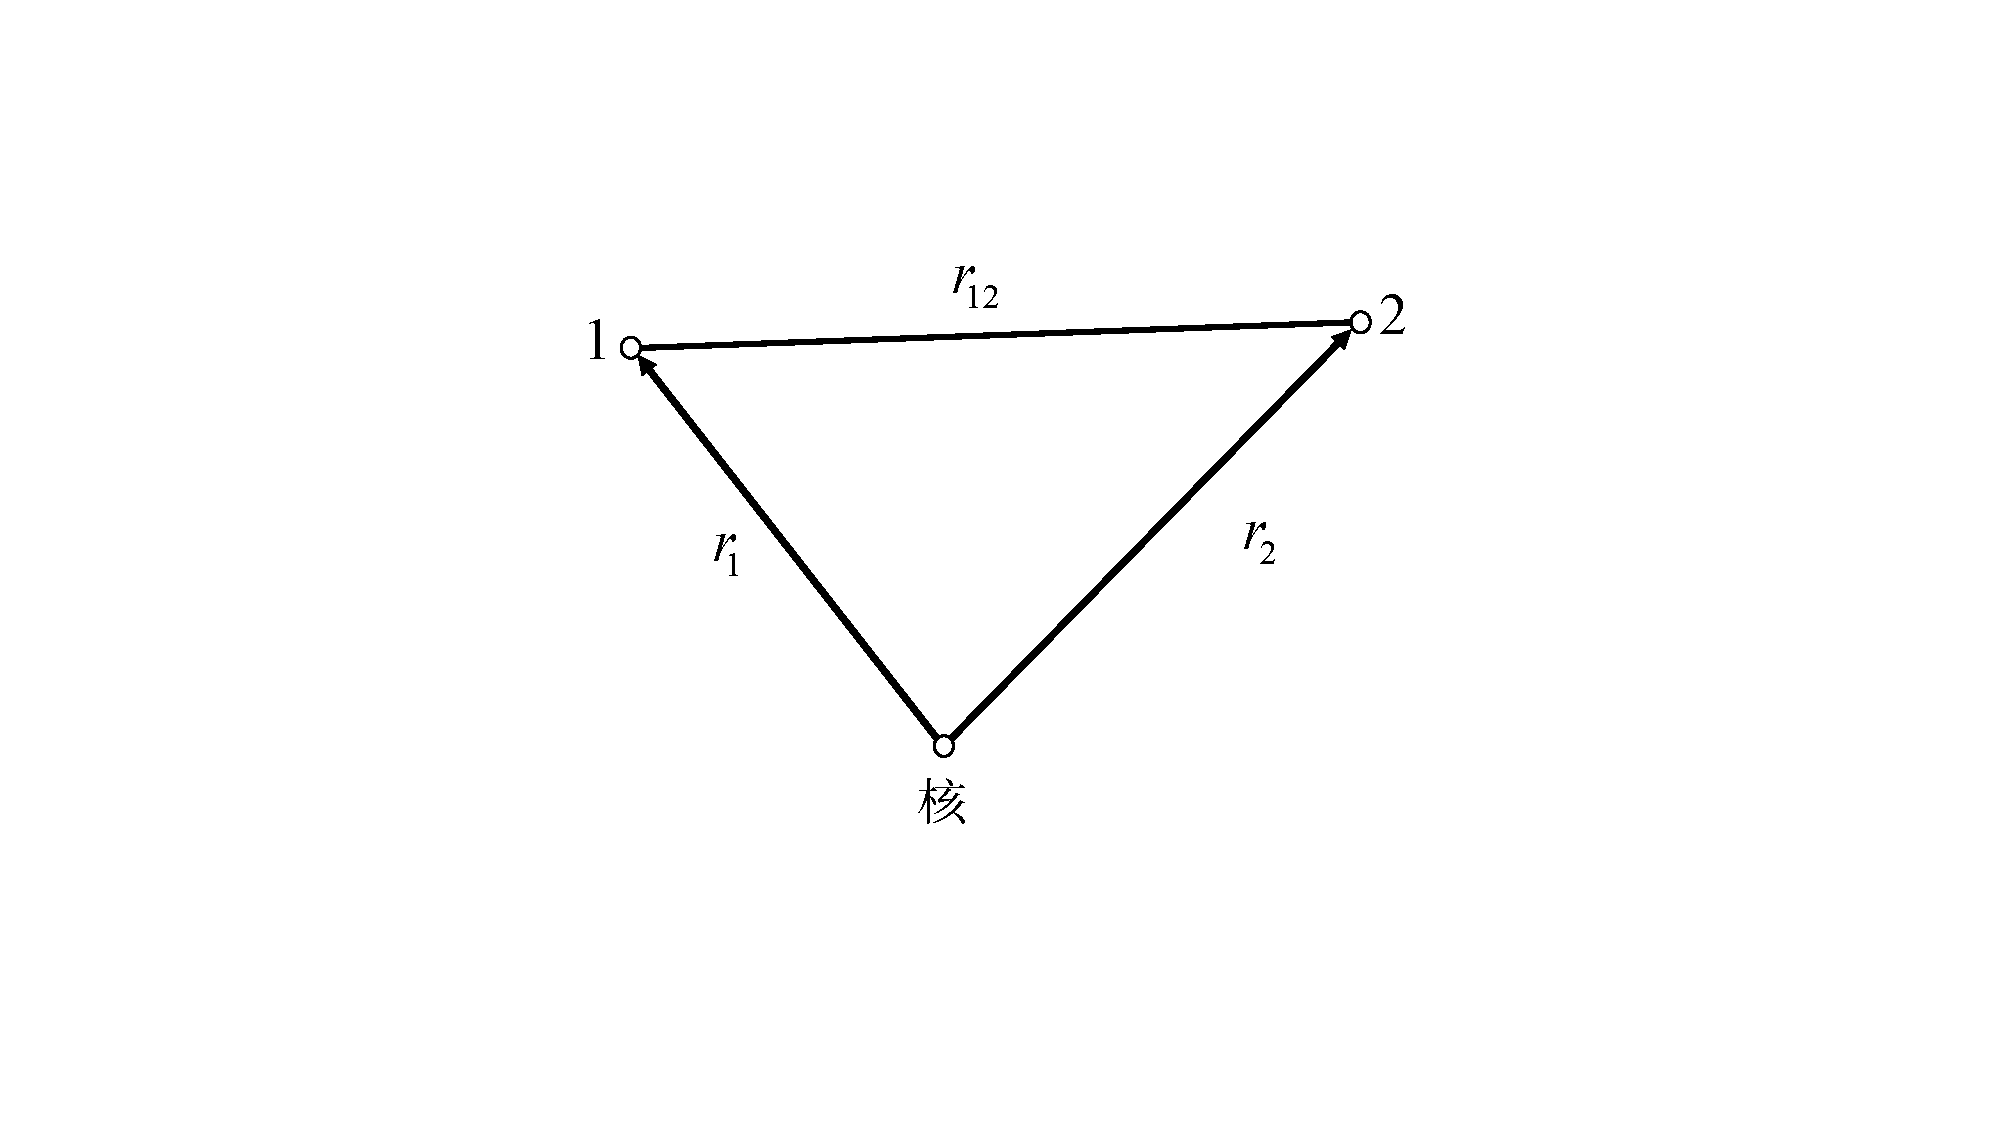
\includegraphics[width=3.5cm,clip]{QM file/figure/10-1}
	\caption{}\label{fig.10-1}
\end{wrapfigure}
这里略去了自旋-轨道耦合作用.


{\heiti 1. 正氦与仲氦}

体系的能级由定态薛定谔方程
\begin{empheq}{equation}\label{eqx3.2}
	H\Psi=E\Psi
\end{empheq}\eqllong
决定.由于$H$不含自旋变量,$\Psi$可以分离变量地表示成
\begin{equation}\label{eqx3.3}
	\Psi(q_{1},q_{2})=\varPsi(\boldsymbol{r}_{1},\boldsymbol{r}_{2})\chi(S_{1z},S_{2z})
\end{equation}\eqnormal
$\varPsi$为“轨道”波函数,$\chi$为自旋波函数.显然,$\varPsi$应该是$H$的本征函数,而$\chi$则与能级没有直接关系.

作为全同费密子体系的波函数,$\Psi$应该具有交换反对称性,即
\begin{empheq}{equation*}
	\hat{P}_{12}\Psi=(\hat{P}_{12}\varPsi)(\hat{P}_{12}\chi)=-\Psi=-\varPsi\chi
\end{empheq}\eqindent{1}
有两种可能的配合:
\begin{empheq}{align}
&(\si{i})	&&\hat{P}_{12}\varPsi=-\varPsi,\qquad \hat{P}_{12}\chi=\chi	\label{eqx3.4}\\
&(\si{ii})	&&\hat{P}_{12}\varPsi=\varPsi,\qquad \hat{P}_{12}\chi=-\chi	\label{eqx3.5}
\end{empheq}\eqnormal
第一种情形轨道波函数$\varPsi$是交换反对称的,自旋波函数则是交换对称的.第二种情形刚好相反.

二电子体系的自旋波函数共有4种(参看$\S$\ref{sec:07.08}),交换对称态有3种,即$\chi_{11},\chi_{10},\chi_{1-1}$,反对称态只有1种,即$\chi_{00}$.对称态相应于总自旋$S=1$,反对称态相应于$S=0$通常将氦原子按其自旋状态分类,称为正氦和仲氦:

正氦:$S=1,\chi=\chi_{11},\chi_{10},\chi_{1-1},\varPsi(\boldsymbol{r}_{1},\boldsymbol{r}_{2})$反对称

仲氦:$S=0,\chi=\chi_{00},\varPsi(\boldsymbol{r}_{1},\boldsymbol{r}_{2})$对称

\noindent 从表面上看,能级仅与$\varPsi(\boldsymbol{r}_{1},\boldsymbol{r}_{2})$有关,与$\chi$无直接关系.但因$\varPsi,\chi$的交换对称性互相制约,而$\varPsi$的交换对称性直接影响到体系的能量.[如$\varPsi$为反对称,$\varPsi(\boldsymbol{r}_{1},\boldsymbol{r}_{2})=-\varPsi(\boldsymbol{r}_{2},\boldsymbol{r}_{1})$,当$\boldsymbol{r}_{1}=\boldsymbol{r}_{2}$,$\varPsi=0$,因此两电子位置接近的概率较小,从而$\frac{\e^{2}}{r_{12}}$的平均值偏小.如$\varPsi$为交换对称,就没有这种性质.]所以正氦与仲氦将具有不同的能级.正氦的每一个能级都相应于自旋三重态,仲氦能级相应于自旋单态.

{\heiti 2. 微扰论} 

将两电子的相互作用势$\frac{\e^{2}}{r_{12}}$当作微扰,\eqref{eqx3.1}式可以表示成
\begin{empheq}{equation}\label{eqx3.6}
	H=H_{0}(\boldsymbol{r}_{1})+H_{0}(\boldsymbol{r}_{2})+H^{\prime}
\end{empheq}\eqlong
其中
\begin{empheq}{equation}\label{eqx3.7}
	H^{\prime}=\frac{\e^{2}}{r_{12}},\quad H_{0}(\boldsymbol{r}_{i})=-\frac{\hbar^{2}}{2m_{e}}\nabla_{i}^{2}-\frac{2\e^{2}}{r_{i}}\quad(i=1,2)
\end{empheq}\eqnormal
$H_{0}(\boldsymbol{r}_{i})$的本征值与本征函数就是类氢离子$(Z=2)$的能级与波函数
\begin{empheq}{equation}\label{eqx3.8}
	E_{n}=-\frac{4\e^{2}}{2n^{2}a_{0}},\quad \varPsi_{nlm}=R_{nl}Y_{lm}
\end{empheq}\eqlong
按照微扰论,轨道波函数的零级近似应该是$H_{0}(\boldsymbol{r}_{1})+H_{0}(\boldsymbol{r}_{2})$的本征函数,其一般形式为
\begin{empheq}{equation}\label{eqx3.9}
	\varPsi_{nlm}(\boldsymbol{r}_{1})\varPsi_{n^{\prime}l^{\prime}m^{\prime}}(\boldsymbol{r_{2}}),\quad \varPsi_{n^{\prime}l^{\prime}m^{\prime}}(\boldsymbol{r}_{1})\varPsi_{nlm}(\boldsymbol{r}_{2})
\end{empheq}\eqlllong
相应于能级(零级近似)$E_{n}+E_{n^{\prime}}$.在以下的叙述中,量子数$nlm$将简记成$n$.作为二电子体系的轨道波函数,应该具有交换对称或反对称性,显然应取下列形式:
\begin{empheq}{equation}\label{eqx3.10}
	\begin{aligned}
		\varPsi_{nn}^{S}(\boldsymbol{r}_{1},\boldsymbol{r}_{2}) &=\varPsi_{n}(\boldsymbol{r}_{1})\varPsi_{n}(\boldsymbol{r}_{2})	\\
		\varPsi_{nn^{\prime}}^{S}(\boldsymbol{r}_{1},\boldsymbol{r}_{2})	 &=\frac{1}{\sqrt{2}}[\varPsi_{n}(\boldsymbol{r}_{1})\varPsi_{n^{\prime}}(\boldsymbol{r_{2}})+\varPsi_{n^{\prime}}(\boldsymbol{r}_{1})\varPsi_{n}(\boldsymbol{r}_{2})]\quad (n\neq n^{\prime})		\\
		\varPsi_{nn^{\prime}}^{A}(\boldsymbol{r}_{1},\boldsymbol{r}_{2}) &=\frac{1}{\sqrt{2}}[\varPsi_{n}(\boldsymbol{r}_{1})\varPsi_{n^{\prime}}(\boldsymbol{r_{2}})-\varPsi_{n^{\prime}}(\boldsymbol{r}_{1})\varPsi_{n}(\boldsymbol{r}_{2})]\quad (n\neq n^{\prime})
	\end{aligned}
\end{empheq}\eqlong
由于微扰$H^{\prime}=\frac{\e^{2}}{r_{12}}$是交换对称的,必然有
\begin{empheq}{equation}\label{eqx3.11}
	\langle \varPsi^{S}|H^{\prime}|\varPsi^{A}\rangle=\iint\varPsi^{S*}\frac{\e^{2}}{r_{12}}\varPsi^{A}d\tau_{1}d\tau_{2}=0
\end{empheq}\eqnormal
(在上式中交换$\boldsymbol{r}_{1},\boldsymbol{r}_{2}$,相当于$\boldsymbol{r}_{1}$改写成$\boldsymbol{r}_{2}$,$\boldsymbol{r}_{2}$改写成$\boldsymbol{r}_{1}$,对于积分值显然没有影响.但这样做时,$\varPsi^{S}$,$\frac{\e^{2}}{r_{12}}$不变,$\varPsi^{A}$则要变号,因此积分值要变号.由此可知积分值必为.)按照简并化微扰论,既然微扰$H^{\prime}$并不造成对称态与反对称态间的耦合,能级的一级修正就等于$H^{\prime}$的平均值,记为
\begin{empheq}{equation}\label{eqx3.12}
	\begin{aligned}
		E_{nn}^{S} &= \langle \varPsi_{nn}^{S}|\frac{\e^{2}}{r_{12}}|\varPsi_{nn}^{S} \rangle 	\\
		E_{nn^{\prime}}^{S} &= \langle \varPsi_{nn^{\prime}}^{S}|\frac{\e^{2}}{r_{12}}|\varPsi_{nn^{\prime}}^{S} \rangle 	\\
		E_{nn^{\prime}}^{A} &= \langle \varPsi_{nn^{\prime}}^{S}|\frac{\e^{2}}{r_{12}}|\varPsi_{nn^{\prime}}^{A} \rangle 	
	\end{aligned}
\end{empheq}
显然
\begin{empheq}{align}\label{eqx3.13}
	E_{nn}^{S} &=\iint\frac{\e^{2}}{r_{12}}|\varPsi_{n}(\boldsymbol{r}_{1})|^{2}|\varPsi_{n}(\boldsymbol{r}_{2})|^{2}d\tau_{1}d\tau_{2}	\nonumber\\
	&\equiv C(n,n)
\end{empheq}
这是电子1,2均处于轨道态$\varPsi_{n}$时,它们之间的库仑作用势的平均值.对于\eqref{eqx3.12}式的后二式,可以算出
\begin{empheq}{align}
	E_{nn^{\prime}}^{S} &=C(n,n^{\prime})+J(n,n^{\prime})	\label{eqx3.14}\\
	E_{nn^{\prime}}^{A} &=C(n,n^{\prime})-J(n,n^{\prime})	\label{eqx3.15}
\end{empheq}\eqlong
其中
\begin{empheq}{align}
	C(n,n^{\prime}) &=\iint\frac{\e^{2}}{r_{12}}|\varPsi_{n}(\boldsymbol{r}_{1})|^{2}|\varPsi_{n^{\prime}}(\boldsymbol{r}_{2})|^{2}d\tau_{1}d\tau_{2}	\nonumber\\
	&=\iint\frac{\e^{2}}{r_{12}}|\varPsi_{n^{\prime}}(\boldsymbol{r}_{1})|^{2}|\varPsi_{n}(\boldsymbol{r}_{2})|^{2}d\tau_{1}d\tau_{2}		\label{eqx3.16}\\
	J(n,n^{\prime}) &=\iint\frac{\e^{2}}{r_{12}}\varPsi_{n}^{*}(\boldsymbol{r}_{1})\varPsi_{n^{\prime}}(\boldsymbol{r}_{1})\varPsi_{n^{\prime}}^{*}(\boldsymbol{r}_{2})\varPsi_{n}(\boldsymbol{r}_{2})d\tau_{1}d\tau_{2}	\label{eqx3.17}
\end{empheq}
习惯上称$C(n,n^{\prime})$为“库仑能”,称$J(n,n^{\prime})$为“交换能”,其实它们都是两电子间库仑作用势$\frac{\e^{2}}{r_{12}}$平均值的一部分.从形式上看,$C(n,n^{\prime})$相当于一个电子处于$\varPsi_{n}$态,另一个电子处于$\varPsi_{n^{\prime}}$态时$\frac{\e^{2}}{r_{12}}$的平均值.$J(n,n^{\prime})$则没有这样直观简单的解释,它是两个电子交换其单电子态的产物,根源在于波函数的交换对称性.

总结上述计算,准确到微扰论一级近似,氦原子能级为:

正氦($S=1$,$\varPsi$反对称)
\begin{empheq}{equation}\label{eqx3.18}
	E=E_{n}+E_{n^{\prime}}+C(n,n^{\prime})-J(n,n^{\prime})\quad (n\neq n^{\prime})
\end{empheq}

仲氦($S=0$,$\varPsi$对称)
\begin{empheq}{align}
	E&=2E_{n}+C(n,n)\quad (n=n^{\prime})		\label{eqx3.19}\\
	E&=E_{n}+E_{n^{\prime}}+C(n,n^{\prime})+J(n,n^{\prime})\quad (n\neq n^{\prime})	\label{eqx3.20}
\end{empheq}\eqnormal
$C(n,n^{\prime})$与$J(n,n^{\prime})$的计算相当繁,从略.当$n,n^{\prime}$较小时,$C$与$J$均为正,但$J(n,n^{\prime})<C(n,n^{\prime})$,所以当$n\neq n^{\prime}$,正氦和仲氦能级接近,仲氦稍高.但仲氦还有$n=n^{\prime}$(两个电子处于相同状态)的能级,即\eqref{eqx3.19}式.氦原子的低激发态,一个电子处于最低的$E_{1}$能级($\varPsi_{100}$态),另一个电子处于$E_{n}$能级($\varPsi_{nlm}$态,$n\geqslant2$),由于$\varPsi_{100}$与$\varPsi_{nlm}$重叠较少,因此交换能$J(100,nlm)$显得微不足道.只有当两个电子同处一个壳层($n$相同,$lm\neq l^{\prime}m^{\prime}$),空间位置较接近,交换能才变得重要.

{\heiti 3. 基态(微扰论及变分法)} 

氦原子的基态属于仲氦,两个电子同处轨道态$\varPsi_{100}$,总自旋为0.按照微扰论,轨道波函数(零级近似)为
\begin{empheq}{equation}\label{eqx3.21}
	\varPsi_{100,100}^{S}(r_{1},r_{2})=\varPsi_{100}(r_{1})\varPsi_{100}(r_{2})
\end{empheq}
其中$\varPsi_{100}$为类氢离子$(Z=2)$基态波函数,即
\begin{empheq}{equation}\label{eqx3.22}
	\varPsi_{100}(r)=\left(\frac{8}{\pi a_{0}^{3}}\right)^{\frac{1}{2}}e^{-2r/a_{0}}
\end{empheq}
利用公式
\begin{empheq}{equation}\label{eqx3.23}
	\iint\frac{1}{r_{12}}e^{-\alpha(r_{1}+r_{2})}d\tau_{1}d\tau_{2}=\frac{20\pi^{2}}{\alpha^{5}}\quad (\alpha>0)
\end{empheq}
(证明见本节末)容易算出
\begin{empheq}{equation}\label{eqx3.24}
	C(100,100)=\frac{5}{4}\cdot\frac{\e^{2}}{a_{0}}
\end{empheq}\eqlong
因此氦原子基态能量的微扰论结果为
\begin{empheq}{equation}\label{eqx3.25}
	E_{0}(\text{微扰论})=2E_{1}+C(100,100)=-\num{2.75}\frac{\e^{2}}{a_{0}}
\end{empheq}\eqnormal
实验值则是
\begin{empheq}{equation*}
	E_{0}(\text{实验})=-\num{79.01}\si{eV}=-\num{2.9037}\frac{\e^{2}}{a_{0}}
\end{empheq}
二者约相差5.3\%.

在上述微扰论计算中,电子的轨道波函数\eqref{eqx3.22}式描述的是电子在原子核所生库仑场中的运动,忽略了另一个电子的存在所产生的影明.事实上,另一个电子的存在,将在一定程度上对核电荷起屏蔽作用,每一个电子感受到的总库仑势(原子核及另一个电子的库仑势之和)粗略地等效于电荷$\lambda e(1<\lambda<2)$产生的库仑势如改用变分法计算,就可以反映这种屏蔽效应.取变分试探函数
\begin{empheq}{align}\label{eqx3.26}
	\varPsi(\lambda,r_{1},r_{2}) &=\varPsi(\lambda,r_{1})\varPsi(\lambda,r_{2})	\nonumber\\
	&=\frac{\lambda^{3}}{\pi a_{0}^{3}}e^{-\lambda r_{1}/a_{0}}e^{-\lambda r_{2}/a_{0}}
\end{empheq}
作为氦原子基态轨道波函数的近似,其中$\lambda$为变分参数.上式已经归一化.当$\lambda=2$,上式就是\eqref{eqx3.21}式.

对\eqref{eqx3.26}式计算总能量H的平均值,即
\begin{empheq}{equation*}
	E(\lambda)=\langle\varPsi(\lambda,r_{1},r_{2})|H|\varPsi(\lambda,r_{1},r_{2})\rangle 
\end{empheq}\eqlong
容易求得
\begin{empheq}{align}
	\langle\nabla_{1}^{2}\rangle =&\langle\nabla_{2}^{2}\rangle=\int\varPsi(\lambda,r)\nabla^{2}\varPsi(\lambda,r)d\tau	\nonumber\\
	=&-\int|\nabla\varPsi(\lambda,r)|^{2}d\tau=-\left(\frac{\lambda}{a_{0}}\right)-\nonumber \\
	&\frac{\hbar^{2}}{2m_{e}}\langle\nabla_{1}^{2}+\nabla_{2}^{2}\rangle=\frac{\hbar^{2}\lambda^{2}}{m_{e}a_{0}}=\lambda^{2}\frac{\e^{2}}{a_{0}} \label{eqx3.27}\\
	\left\langle\frac{1}{r_{1}}\right\rangle=&\left\langle\frac{1}{r_{2}}\right\rangle=\int\frac{1}{r}\varPsi^{2}(\lambda,r)d\tau=\frac{\lambda}{a_{0}}-\nonumber\\& 2\e^{2}\left\langle\frac{1}{r_{1}}+\frac{1}{r_{2}}\right\rangle=-4\lambda\frac{\e^{2}}{a_{0}}		\label{eqx3.28}\\
	\left\langle\frac{\e^{2}}{r_{12}}\right\rangle=&\e^{2}\iint\frac{1}{r_{12}}\varPsi^{2}(\lambda,r_{1})\varPsi^{2}(\lambda,r_{2})d\tau_{1}d\tau_{2}	\nonumber\\
	=&\frac{5\lambda}{8}\frac{\e^{2}}{a_{0}}		\label{eqx3.29}
\end{empheq}\eqnormal
因此
\begin{empheq}{equation}\label{eqx3.30}
	E(\lambda)=\left(\lambda^{2}-\frac{27}{8}\lambda\right)\frac{\e^{2}}{a_{0}}
\end{empheq}
由极值条件$\frac{\partial E(\lambda)}{\partial\lambda}$.求得$\lambda$的最佳值为$\lambda_{0}=\frac{27}{16}$.所以基态能级的变分法结果为
\begin{empheq}{equation}\label{eqx3.31}
	E(\lambda_{0})=-\left(\frac{27}{16}\right)^{2}\frac{\e^{2}}{a_{0}}=-\num{2.8477}\frac{\e^{2}}{a_{0}}
\end{empheq}
这结果比实验值略高,二者相差1.93\%.与微扰论结果相比,变分法结果已大有改进.如果试探波函数的构造再复杂一些,结果还可以改善,直到与实验值完全符合.由此可见,量子力学理论辅以恰当的数学方法,可以成功地处理原子构造问题.

\eqref{eqx3.23}式的证明如下.将积分写成
\begin{empheq}{equation*}
	I-\iint d\tau_{2}I_{1}e^{-\alpha r_{2}},\quad I_{1}=\int\frac{1}{r_{12}}e^{-\alpha r_{1}}d\tau_{1}
\end{empheq}
计算$I_{1}$时,取$\boldsymbol{r}_{2}$为极轴(参看图\ref{fig.10-2}),$\boldsymbol{r}_{1}$用球坐标,则
\begin{empheq}{align*}
	d\tau_{1}&=r_{1}^{2}dr_{1}\sin\theta d\theta d\varphi	\\
	r_{12}&=(r_{1}^{2}+r_{2}^{2}-2r_{1}r_{2}\cos\theta)^{\frac{1}{2}}
\end{empheq}\eqindent{3}
\begin{wrapfigure}[6]{r}{5em}
	\centering
	\small
	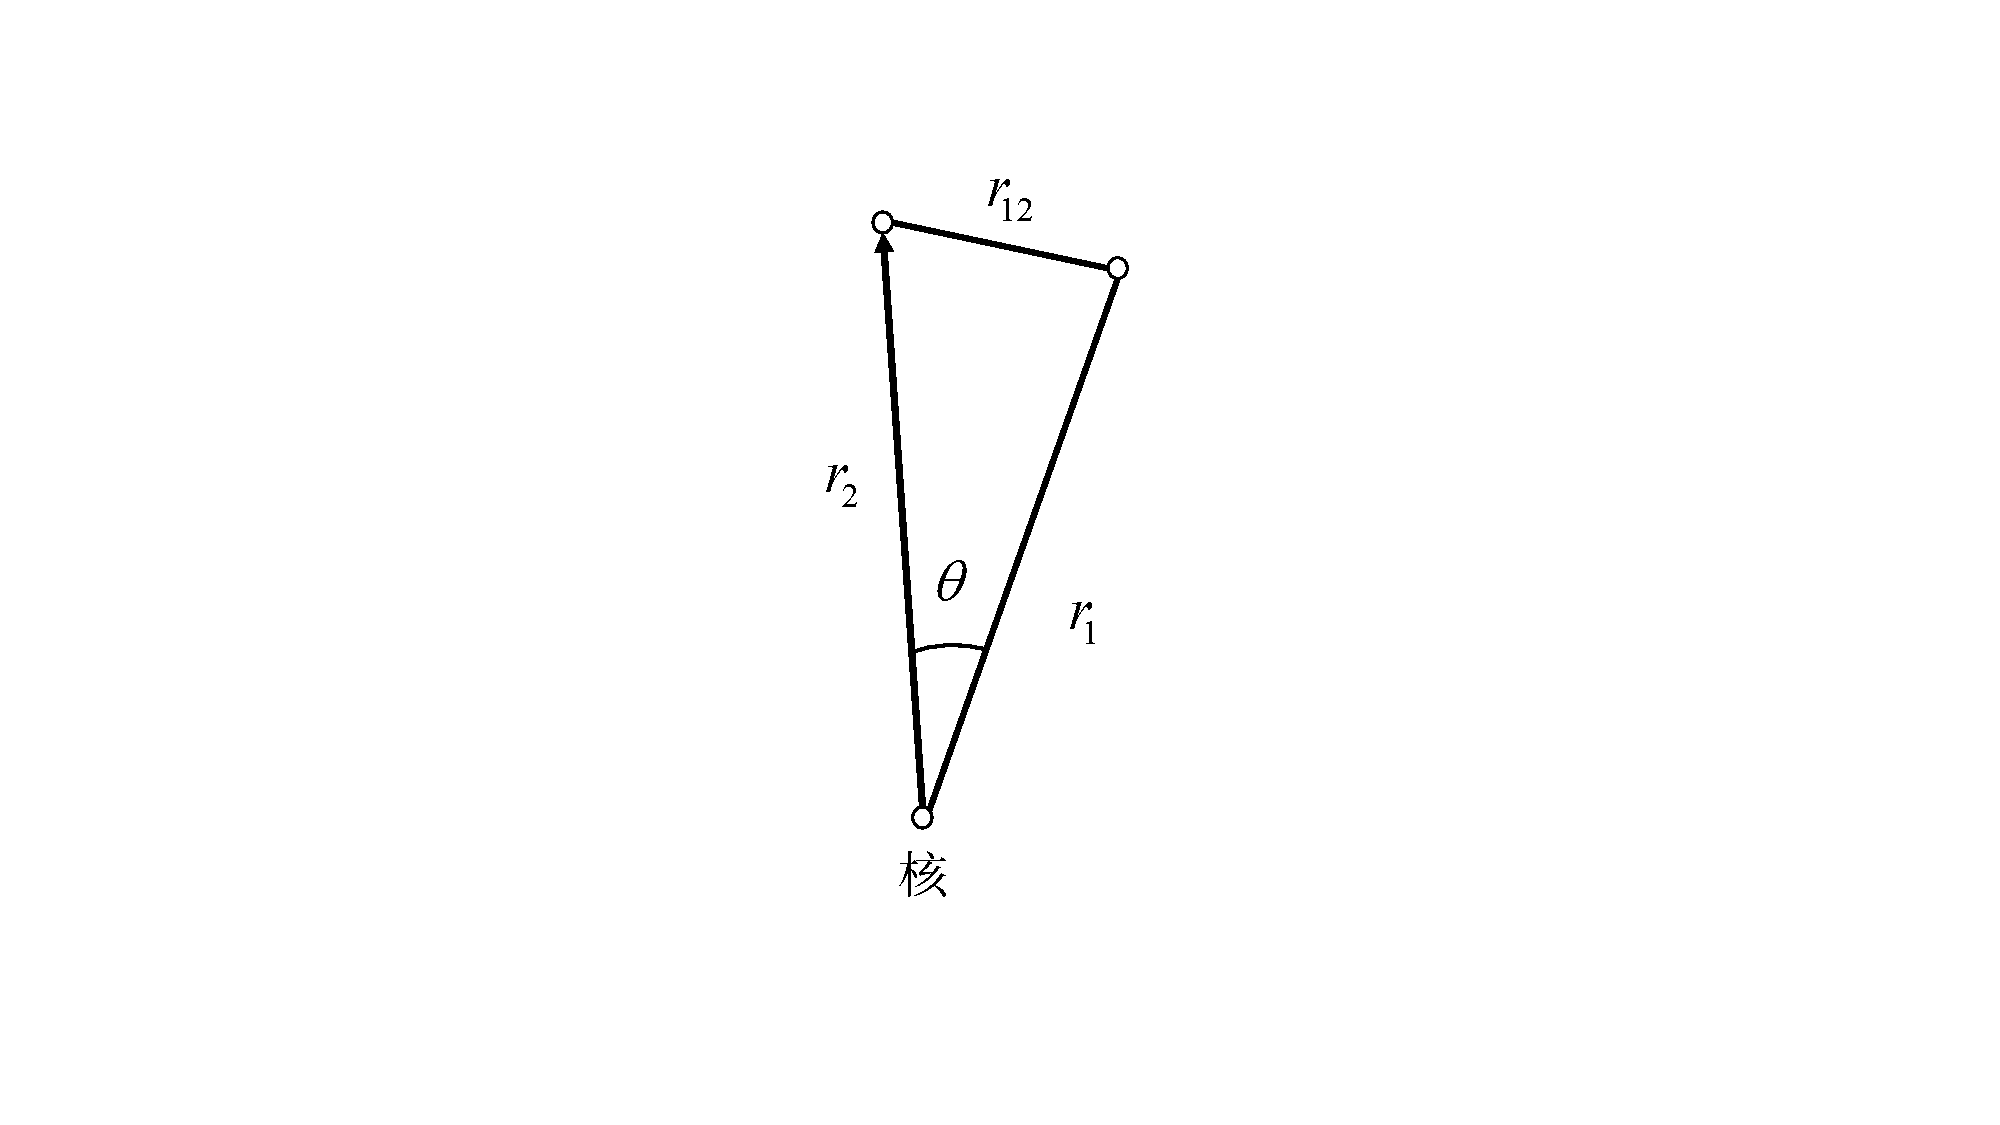
\includegraphics[width=2cm,clip]{QM file/figure/10-2}
	\caption{}\label{fig.10-2}
\end{wrapfigure}
容易算出
\begin{empheq}{equation*}
	I_{1}=\int_{0}^{\infty}dr_{1}r_{1}^{2}e^{-\alpha r_{1}}2\pi\int_{0}^{\pi}(r_{1}^{2}+r_{2}^{2}-2r_{1}r_{2}\cos\theta)^{\frac{1}{2}}\sin\theta d\theta
\end{empheq}\eqlong
其中
\begin{empheq}{align*}
	&\int_{0}^{\pi}(r_{1}^{2}+r_{2}^{2}-2r_{1}r_{2}\cos\theta)^{\frac{1}{2}}\sin\theta d\theta	\\
	=&\frac{1}{r_{1}r_{2}}(r_{1}^{2}+r_{2}^{2}-2r_{1}r_{2}\cos\theta)^{\frac{1}{2}}\bigg|_{\theta=0}^{\theta=\pi} \\
	=&\frac{1}{r_{1}r_{2}}[(r_{1}+r_{2})-|r_{1}-r_{2}|]	\\
	=&\begin{dcases}
		\frac{2}{r_{2}},\quad r_{1}<r_{2}	\\
		\frac{2}{r_{1}},\quad r_{1}>r_{2}
	\end{dcases}	
\end{empheq}
因此
\begin{empheq}{align*}
	I_{1}=&4\pi\int_{0}^{r_{2}}\frac{1}{r_{2}}r_{1}^{2}e^{-\alpha r_{1}}dr_{1}+4\pi\int_{r_{2}}^{\infty}r_{1}e^{-\alpha r_{1}}dr_{1}	\\
	&=\frac{4\pi}{\alpha^{2}}\left[ \frac{2}{\alpha r_{2}}-\left(1+\frac{2}{\alpha r_{2}}\right)e^{-\alpha r_{2}} \right]
\end{empheq}
代入$I$中,即得
\begin{empheq}{align*}
	I&=r\pi\int_{0}^{\infty}I_{1}e^{-\alpha r_{2}}r_{2}^{2}dr_{2}	\\
	&=\frac{16\pi^{2}}{\alpha^{5}}\int_{0}^{\infty}x^{2}e^{-x}\left[\frac{2}{x}-\left(1+\frac{2}{x}\right)e^{-x} \right]	\\
	&=20\pi^{2}/\alpha^{5}
\end{empheq}\eqnormal
此即\eqref{eqx3.23}式.



